\documentclass[14pt]{extreport}
\usepackage{gost}

\begin{document}

\pagestyle{empty}
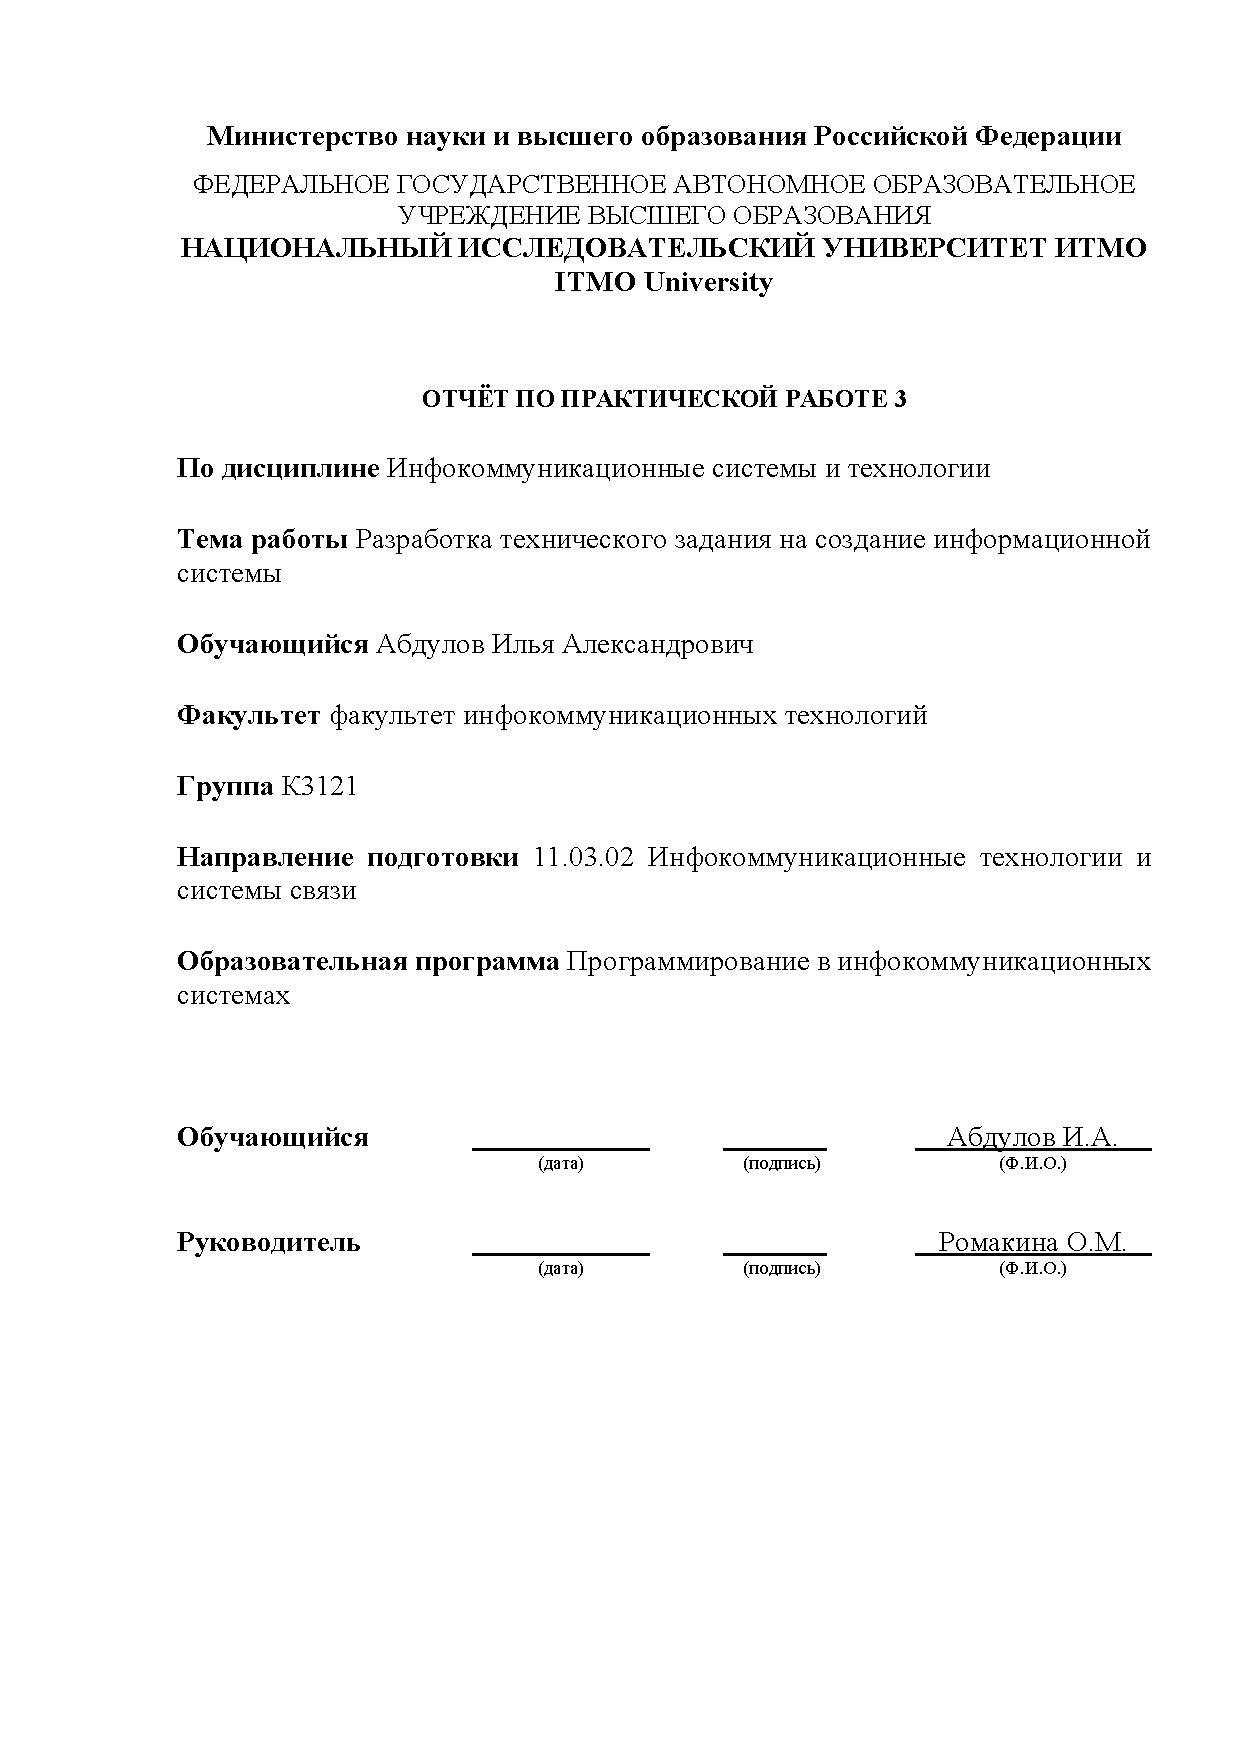
\includepdf{titulCourse.pdf}
\pagestyle{plain}

\tableofcontents

\intro

Практическая работа 7 является актуальной, потому что является описанием основных функциональных элементов будущего мобильного приложения. Приложение Better Row представляет из себя приложение, куда пользователь заносит данные своих тренировок, чтобы приложение показывало и сохраняло текущие показатели и прогресс. Использование приложения придаст тренировкам осознанности, что поможет в достижении лучшего результата.

Целью данной работы является описание предметной области функционирования и построение диаграмм DFD, модели IDEF3 с двумя уровнями декомпозиции, модели процесса в нотации BPMN.

\chapter{Основная часть}

\section{Предметная область функционирования}

Приложение предназначено для развития спортивной деятельности в университете ИТМО, информационная система разрабатывается для клуба по академической гребли. Приложение позволяет сохранять данные о тренировке и всесторонне анализировать их для удобства отслеживания прогресса.

\begin{landscape}
\section{Диаграммы DFD}
\begin{figure}[H]
\centerline{\includegraphics[width=0.73\linewidth]{A-0_DFD_diagram.pdf}}
\caption{Контекстная диаграмма в стандарте DFD}
\label{fig11}
\end{figure}

\begin{figure}[H]
\centerline{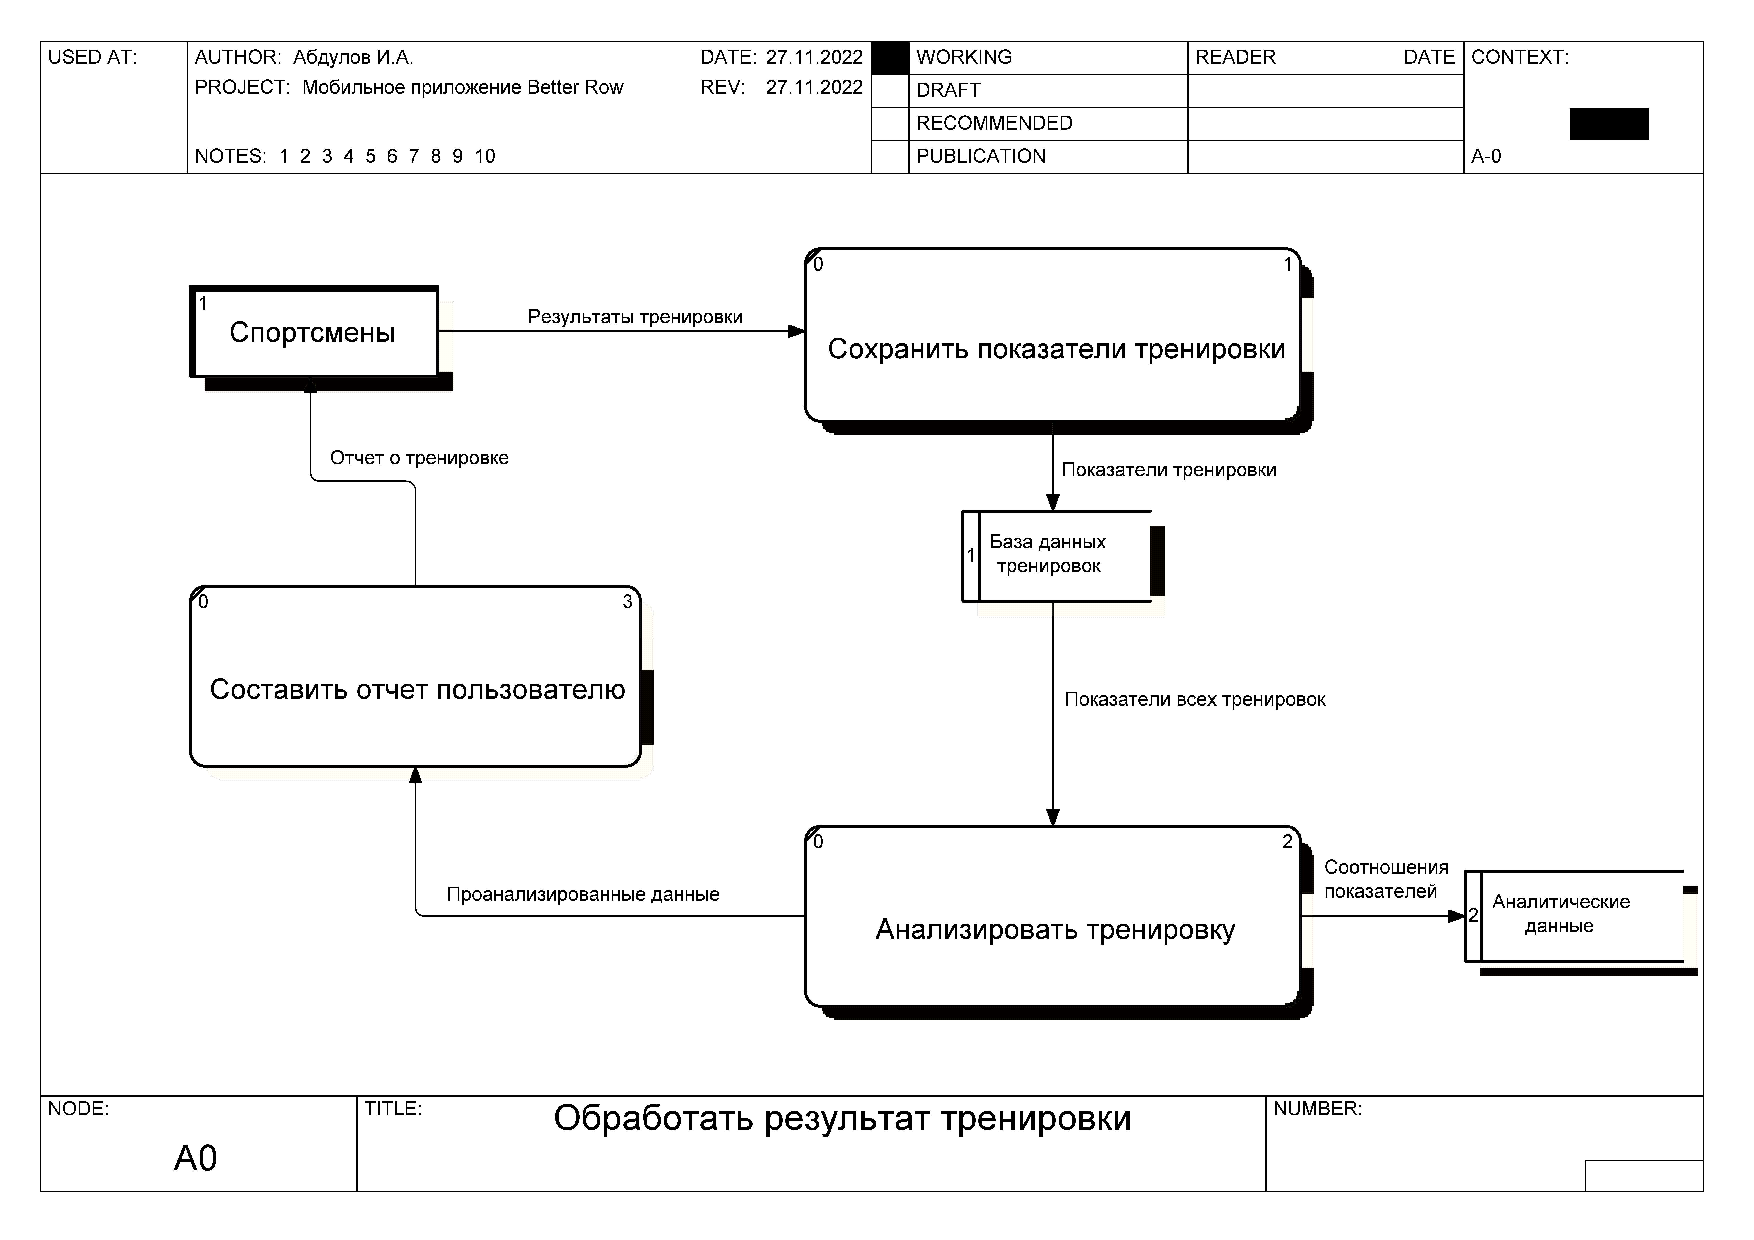
\includegraphics[width=0.8\linewidth]{A0_DFD_diagram.pdf}}
\caption{Декомпозиция блока "Обработать результат тренировки"{} в стандарте DFD}
\label{fig12}
\end{figure}

\section{Модель IDEF3}

\begin{figure}[H]
\centerline{\includegraphics[width=0.73\linewidth]{01_IDEF3.pdf}}
\caption{Блок "Система работы приложения"{} в IDEF3}
\label{fig13}
\end{figure}

\begin{figure}[H]
\centerline{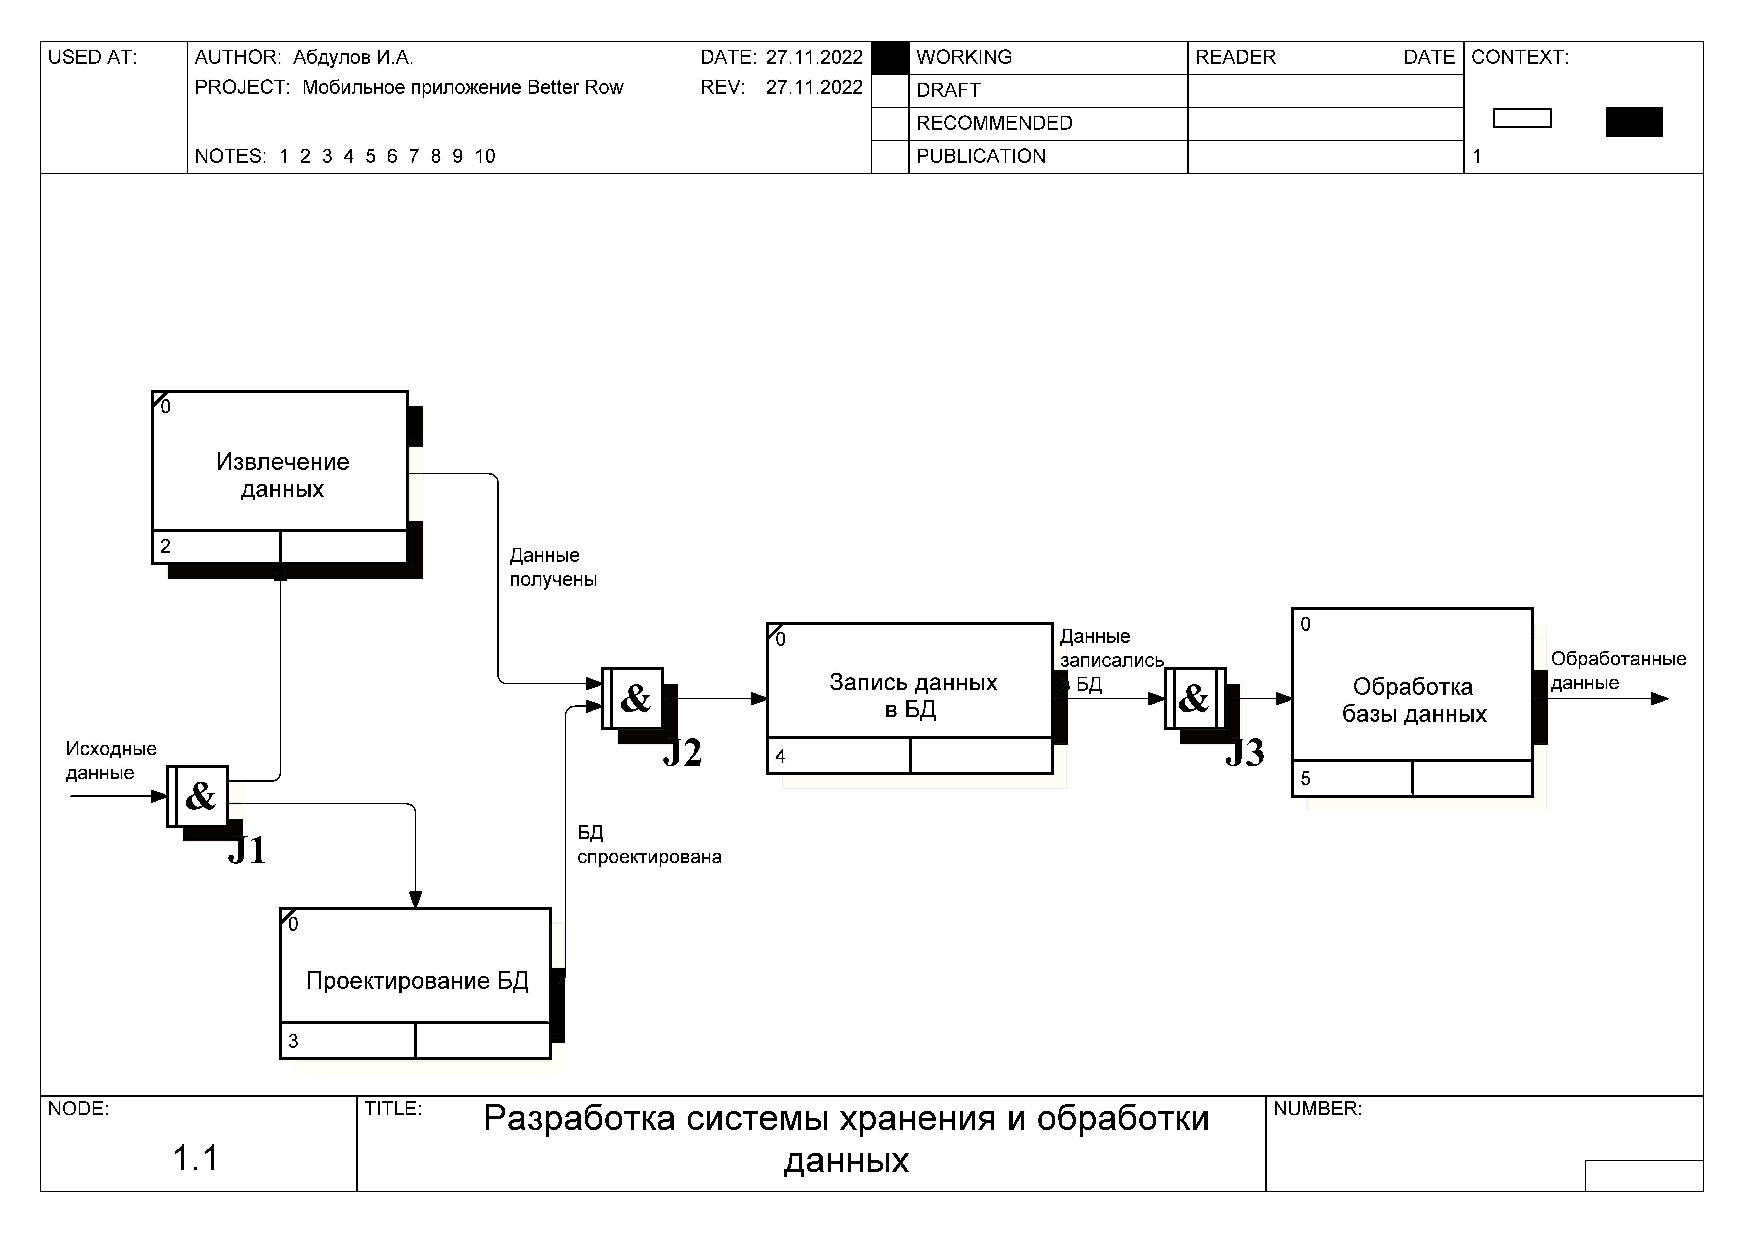
\includegraphics[width=0.8\linewidth]{1-1_IDEF3.pdf}}
\caption{Декомпозиция блока "Разработка системы хранения и обработки данных"{} в IDEF3}
\label{fig14}
\end{figure}

\begin{figure}[H]
\centerline{\includegraphics[width=0.8\linewidth]{5-1_IDEF3.pdf}}
\caption{Декомпозиция блока "Обработка базы данных"{} в IDEF3}
\label{fig15}
\end{figure}

\section{Модель процесса в нотации BPMN}

\begin{figure}[H]
\centerline{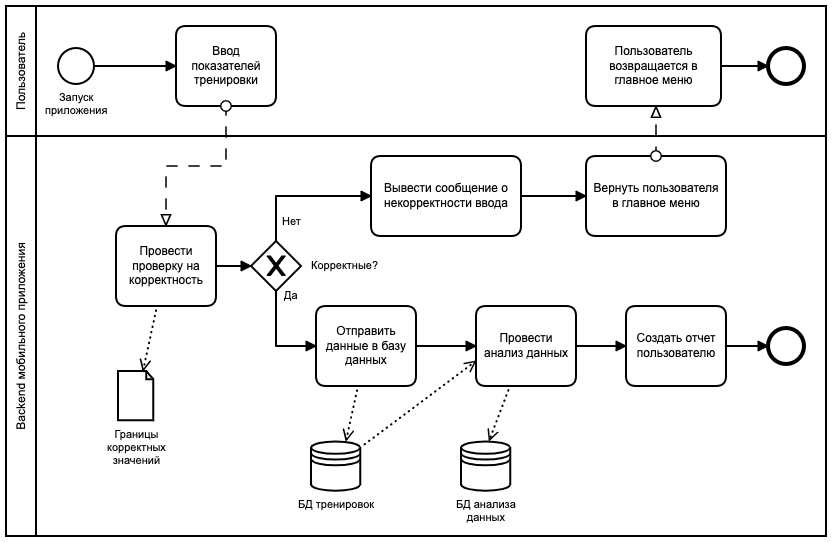
\includegraphics[width=0.73\linewidth]{BPMN.jpg}}
\caption{Модель процесса запуска приложения в нотации BPMN}
\label{fig16}
\end{figure}

\end{landscape}

\conclusions

Цель работы была достигнута. Была описана предметная область функционирования мобильного приложения. В отчёте были представлены построенные диаграммы потоков данных DFD, модели IDEF3 с двумя уровнями декомпозиции, модели процесса в нотации BPMN.

\newpage
\begin{thebibliography}{99}

\bibitem{bib1}Интернет-статья по построению диаграмм DFD — URL: \url{https://itteach.ru/bpwin/dfd-i-workflow-idef3} (дата обращения 26.11.2022).	

\bibitem{bib2}Интернет-статья по методологии IDEF3 — URL: \url{https://itteach.ru/bpwin/metodologiya-idef3} (дата обращения 26.11.2022).	

\bibitem{bib3}Интернет-приложение для создания моделей процессов BPMN — URL: \url{https://stormbpmn.com/} (дата обращения 27.11.2022).	
	
\end{thebibliography}

\end{document}
